\documentclass[a4paper,11pt,english]{article}

% Basic packages
\usepackage[utf8]{inputenc}
\usepackage{a4wide}
\usepackage{lmodern}
\usepackage[T1]{fontenc}
\usepackage{babel}
\setlength{\parindent}{0pt} 
\setlength{\parskip}{2ex}
\usepackage{fixltx2e}
\usepackage{amsmath, amssymb}
\usepackage[pdftex, pdfborderstyle={/S/U/W 0}]{hyperref}
\usepackage{graphicx}
\usepackage[font=small,labelfont=bf]{caption}
\usepackage{tabularx}
\usepackage{multirow}
\usepackage{xcolor}
\usepackage{siunitx}
\usepackage{amsmath}
\usepackage{xcolor, colortbl}
\usepackage{float}
\usepackage{mathtools}
\usepackage{mdframed}
\usepackage{dirtytalk}
\usepackage{minted}
\usepackage{subfigure}
\usepackage[strings]{underscore}
\usepackage[toc,page]{appendix}
\usepackage[ruled,vlined]{algorithm2e}
\usepackage{booktabs}


\newmdenv[
  backgroundcolor=gray!20,
  topline=false,
  bottomline=false,
  rightline=false,
  leftline=false,
  skipabove=\baselineskip,
  skipbelow=\baselineskip,
]{myframe}




\title{Anomaly Detection in Slide Rail Machines using Autoencoders}
\author{Group 14 \\ Juan David Zapata Cruz, Krisostomus Nova Rahmanto \\ and Kristian Håland}
\date{\today}

\begin{document}


\maketitle

\begin{abstract}

% Acoustic anomaly detection plays a pivotal role in condition-based maintenance of industrial equipment.  
% The key challenge is to identify previously unseen abnormal sounds when only recordings of healthy operation are available during training.  
% This paper documents a replication of Task~2---Unsupervised Detection of Anomalous Sounds from the DCASE~2020 challenge for the slide-rail machine class, using a simplified dataset tailored to the AML course.  
% The core approach is a convolutional autoencoder (CAE) trained on log-Mel spectrogram representations; anomalies are flagged via elevated reconstruction error.  
% The proposed system attains a ROC--AUC of~0.90  on an internal hold-out test set, a substantial gain over a naïve baseline (0.81).  
% Qualitative inspection reveals that the model is particularly sensitive to distorted or missing harmonic structures.
We address unsupervised fault detection for slide-rail machines using the
\textbf{MIMII} dataset released in DCASE\,2020 Task~2.
Log–Mel spectrograms extracted from 2\,370 normal files train two
one-class models: (i) a 1.2 M-parameter convolutional auto-encoder (CAE)
optimised for 50 epochs with MSE, and (ii) a Deep Support Vector Data
Description (Deep-SVDD) network trained for 10 epochs.

On the 1\,101-file test split the CAE achieves
\textbf{AUC = 0.9008} and an
\textbf{F\textsubscript{1} = 0.896} at a reconstruction-error threshold
of 0.12, while Deep-SVDD scores a higher
AUC = 0.9552 but lowers precision to 0.728.
Visual reconstructions confirm that the CAE reproduces normal signals
faithfully and distorts anomalies, explaining its superior
precision–recall balance.

These findings show that a lightweight CAE trained solely on normal data
can detect slide-rail anomalies with near-90 \% AUC and fewer false
alarms than a deeper Deep-SVDD alternative, making it attractive for
edge deployment.

\end{abstract}

\section{Introduction}
\label{sec:Introduction}

For many industrial applications, anomaly detection techniques can be used to timely prevent potential issues and failures that could affect business goals. However, anomalies are rare and unpredictable, making it impractical to gather representative anomalous samples to develop traditional binary classification algorithms. Hence, unsupervised techniques that learn only from normal data become essential. This project focuses on detecting sound anomalies in Slide Rail machines using a Convolutional Autoencoder (CAE).




\section{Dataset and Preprocessing}
\label{sec:Data Analysis and Preparation}


% \subsection{Dataset Details}
% The dataset used in this study is characterised by the following properties.
% \begin{description}
%   \item[Source:] DCASE~2020 Task~2 Development—slide-rail class
%   \item[Size:] $\approx$3 machine IDs
%   \item[Duration per file:] $\sim$10 s mono\;@\;16 kHz
%   \item[Environment:] Real-world factory background noise
% \end{description}
% The data set used for this project consists of 3471 WAV format sound files labelled either as normal or as anomalies, and divided into a development set of 2370 files with only normal labelled files, and a test set of 1101 files which is made of both classes, 300 normal and 801 anomalies. For monitoring the model's performance across epochs, the development set is divided into a training and a validation set using a 90-10 split.

% The labels are inferred from the filenames, which follow the format \textit{normal/anomaly\_id\_id-number\_sample-number.wav}. For example, \textit{anomaly\_id\_00\_00000015.wav} indicates an anomalous sample. 

% ---------- Subsection: Dataset Details ----------
\subsection{Dataset Details}
\vspace{0.2em}
\noindent
\textbf{Source.}  
All recordings originate from the \emph{MIMII} slide–rail subset introduced by Purohit
\textit{et~al.}\ \cite{purohit2019mimii}.  
This subset constitutes one of the machine types distributed as
development data for \textbf{DCASE 2020 Task 2} on unsupervised anomalous–sound
detection in machine condition monitoring.

\noindent
\textbf{Machine IDs and split.}
The corpus contains \emph{exactly three} machine identities (ID~00, 02, 04).
For each ID, only normal recordings are provided for training
(``dev\_train''), whereas both normal and anomalous examples appear in the
evaluation (``dev\_test'') set:

\begin{table}[h]
\centering
\begin{tabular}{lccc}
\toprule
\textbf{ID} & \textbf{Normal (train)} & \textbf{Normal / Anom.\ (test)} & \textbf{Duration} \\
\midrule
00 & 790 & 100 / 356 & 10 s \\
02 & 790 & 100 / 267 & 10 s \\
04 & 790 & 100 / 178 & 10 s \\
\midrule
\textbf{Total} & 2370 & 300 / 801 & \\
\bottomrule
\end{tabular}
\caption{File counts per machine ID (16 kHz mono).}
\label{tab:id_split}
\end{table}

\noindent
\textbf{Recording conditions.}  
Audio was captured with microphones mounted inside a real factory
environment and therefore includes non-stationary background noise.
Each file is ten seconds long, single-channel, and stored as 16-bit
\texttt{.wav} at 16\,kHz.

\noindent
\textbf{File-name convention.}  
Labels are inferred from the canonical naming scheme
\texttt{\{normal$\vert$anomaly\}\_id\_\{ID\}\_\{NNNNNNNN\}.wav}; e.g.,
\texttt{anomaly\_id\_00\_00000015.wav} designates an anomalous
recording of machine ID~00.

\noindent
\textbf{Usage in this work.}  
We adopt the official split: \emph{dev\_train} (normal-only) for model
training, a 10\,\% held-out slice of the same set for parameter
selection, and \emph{dev\_test} for final reporting.  This mirrors the
zero-positive learning scenario mandated by Task 2.


\subsection{Feature Extraction}
The complete preprocessing pipeline is summarised below:

\begin{enumerate}
  \item \textbf{Short-time Fourier transform (STFT)} with a 1024-sample Hann window and a 512-sample hop (approximately 64~ms and 32~ms, respectively) to expose local spectral content.
  \item \textbf{Mel filterbank} with 64 triangular bands spanning 0–8~kHz, reflecting the frequency resolution of human hearing.
  \item \textbf{Logarithmic compression} using the formula \( \log(1 + 10 \times |\mathrm{Mel}|) \) for variance stabilisation and dynamic-range reduction.
  \item \textbf{Per-file min–max normalisation} to the range \([0, 1]\), followed by \textbf{global standardisation} (zero mean, unit variance) based on training statistics.
\end{enumerate}

% Approaching the intended task in the 1D-domain of the provided raw audio signals diminishes anomaly detection capabilities, as this representation does not expose frequency content, which is key for this task as anomalies are often frequency-localized. Instead, to expose this frequency based patterns as well as reducing data complexity and focusing on relevant structure, this raw signals are transformed into spectrograms, specifically to Log-Mel ones, which compose a more aligned representation with human perception. The resulting are normalized to zero mean and unit variance to improve training stability and help the model focus on scale-invariant features, as preserving relative amplitudes is more important than retaining absolute amplitudes.

Raw audio waveforms are first down-sampled to 16~kHz and transformed into time–frequency representations to better expose spectral regularities where anomalies typically manifest.  
Approaching the task directly in the time domain diminishes anomaly detection capability, as raw waveforms do not reveal frequency-localised patterns that are key indicators of malfunctioning behavior.

To obtain a perceptually meaningful and compact representation, we compute 64-band log-Mel spectrograms. A 1024-sample Hann window (\(\approx\)64~ms) with a 512-sample hop (\(\approx\)32~ms) is applied to perform the short-time Fourier transform (STFT).  
This configuration balances temporal acuity and frequency resolution—sufficient, for example, to capture the $\sim$300~ms mechanical cycle of a typical slide operation.

The Mel spectrogram is then compressed using a log transformation to stabilise variance and reduce dynamic range:
\[
X_{d,b} = \log\left(1 + 10 \cdot M_{d,b}\right),
\]
where \( M_{d,b} \) denotes the Mel energy for frame \( d \) and frequency band \( b \).  
Subsequently, each spectrogram is min–max normalised per file, followed by global standardisation using statistics computed from the training set.  
This ensures that gain variations across sessions do not bias the anomaly score, while allowing the model to focus on scale-invariant structure rather than absolute amplitudes.
Figure \ref{fig:LogMel Viz} visualises two normal and two anomalous examples from the two different machines (ID-00 and ID-02):

\begin{figure}
    \centering
    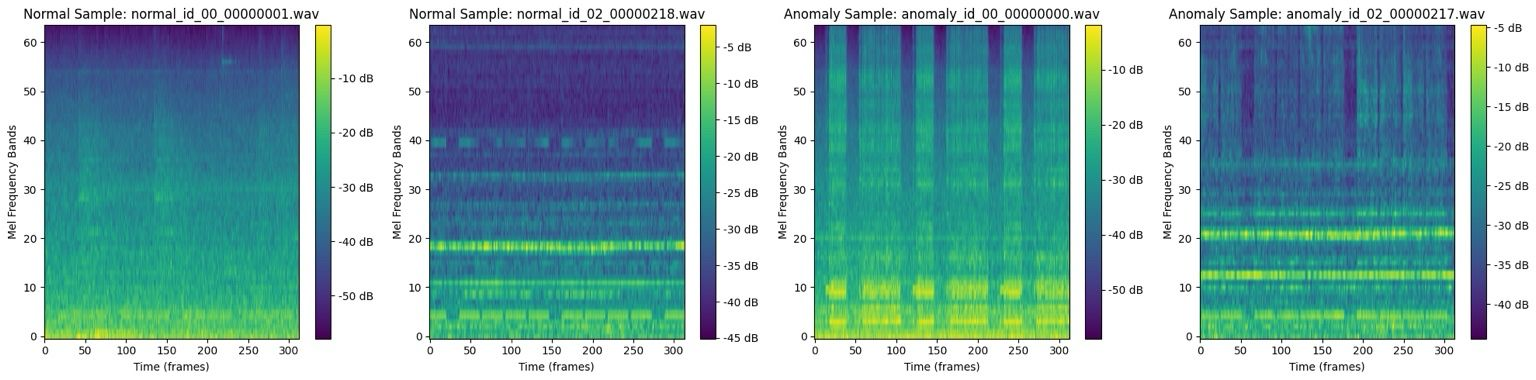
\includegraphics[width=1\linewidth]{Figures/logmel viz.jpeg}
    \caption{Visualization of Mel Spectogram on Normal and Anomaly Machines}
    \label{fig:LogMel Viz}
\end{figure}

% 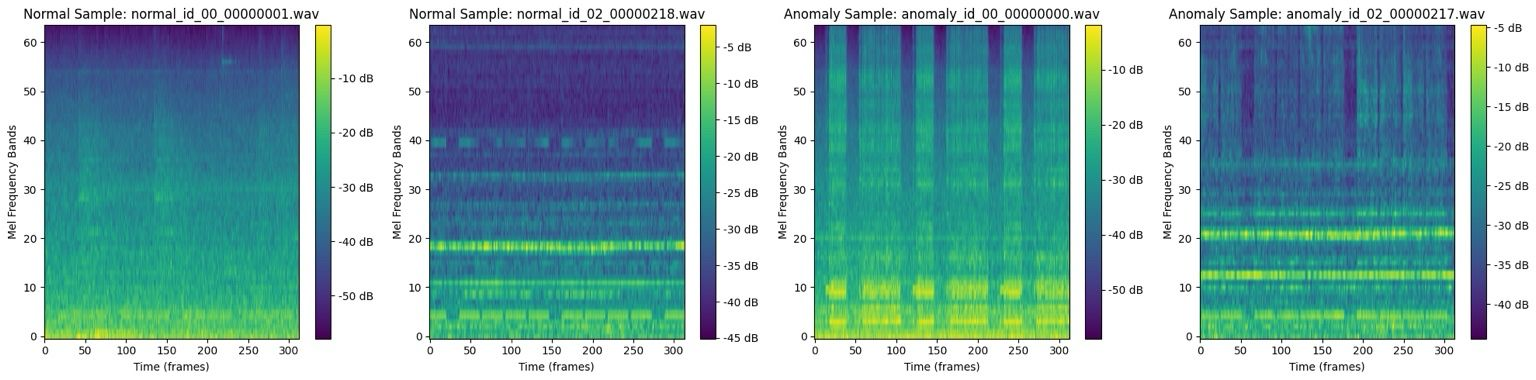
\includegraphics[width=1\textwidth]{Figures/logmel viz.jpeg}
% \label{fig:LogMel Viz}

Figure~\ref{fig:LogMel Viz} shows that anomalous samples notably lack the low-frequency ridges characteristic of healthy operation and exhibit pronounced \emph{vertical stripes} that signal abnormal friction.













\section{Methodology}
\label{sec:Modelling Approach}

The following sections describe the model architecture and training strategy, as well as the reasoning behind them. 

\subsection{Convolutional Autoencoder}
\label{subsec:Model Architecture}
We used convolutional autoencoder(CAE) as our first model. This type of network is composed of two parts, an encoder in charge of compressing the input into a smaller latent representation, and a decoder in charge of reconstructing the original input. When trained with normal samples only, the network learns to perform the reconstruction process just for this type of input; thus, it will fail when reconstructing anomaly samples, generating a higher reconstruction error that exposes the presence of an anomaly.

However, as data now have a grid-like representation, convolutional layers are implemented within the network to exploit their capabilities to capture localized patterns as often anomalies are exposed in specific regions from the frequency domain. Additionally, the convolutional layer parameter sharing feature helps them to detect patterns anywhere in the spectrograms, which makes use of the stationary condition of audio signals and their anomalies. When combined to create deep architectures they can learn composite representations from different levels, from short frequency peaks in a low level scale to engine sounds in a much higher scale.

\textbf{Specifications}

The implemented model uses a symmetric architecture consisting of an encoder and a decoder, connected through a fully connected bottleneck layer in the latent space. The encoder comprises three convolutional layers, each with a kernel size of 3, followed by ReLU activation functions and max-pooling operations for spatial downsampling. The decoder mirrors this structure using transposed convolutional layers to up-sample from the latent representation, again followed by ReLU activations. The model is defined by the pseudocode below:

% \begin{mdframed}[backgroundcolor=gray!20]
% \begin{minted}[breaklines]{python}
% latent_dim=256

% # Encoder
% self.enc = nn.Sequential(
%     nn.Conv2d(1, 16, kernel_size=3, padding=1), nn.ReLU(), 
%     nn.MaxPool2d(2),                   
%     nn.Conv2d(16, 32, kernel_size=3, padding=1), nn.ReLU(),
%     nn.MaxPool2d(2),                   
%     nn.Conv2d(32, 64, kernel_size=3, padding=1), nn.ReLU(),
%     nn.MaxPool2d(2),)

% # Fully connected layers
% self.enc_fc = nn.Sequential(
%     nn.Flatten(), nn.Linear(64 * 8 * 39, latent_dim))

% self.dec_fc = nn.Sequential(
%     nn.Linear(latent_dim, 64 * 8 * 39), nn.Unflatten(1, (64, 8, 39)))

% # Decoder
% self.dec = nn.Sequential(
%     nn.ConvTranspose2d(64, 32, kernel_size=4, stride=2, padding=1), nn.ReLU(),
%     nn.ConvTranspose2d(32, 16, kernel_size=4, stride=2, padding=1), nn.ReLU(),
%     nn.ConvTranspose2d(16, 1, kernel_size=4, stride=2, padding=1),)

% # Final 1x1 conv to pad to 313
% self.pad_to_313 = nn.ConstantPad2d((0, 1, 0, 0), 0)
% \end{minted}
% \end{mdframed}

\begin{algorithm}[H]
\caption{Convolutional Autoencoder with Constant Padding}
\KwData{Log--Mel spectrogram $\mathbf X \in \mathbb{R}^{1 \times 64 \times 313}$}
\KwResult{Reconstructed spectrogram $\hat{\mathbf X}$}

% -------------------------------------------------
% Hyper-parameter
\SetKwComment{tcp}{//}{}
\SetKwProg{Fn}{Function}{}{}
\DontPrintSemicolon

\tcp*[l]{\textbf{Hyper-parameter}}
$\textit{latent\_dim} \leftarrow 256$\;

\BlankLine
% -------------------------------------------------
% Encoder
\tcp*[l]{\textbf{Encoder}}
$\mathbf H \leftarrow \mathrm{Conv2D}(1,16,3,1)\!\circ\!\mathrm{ReLU}\!\circ\!\mathrm{MaxPool2D}(2)(\mathbf X)$\;
$\mathbf H \leftarrow \mathrm{Conv2D}(16,32,3,1)\!\circ\!\mathrm{ReLU}\!\circ\!\mathrm{MaxPool2D}(2)(\mathbf H)$\;
$\mathbf H \leftarrow \mathrm{Conv2D}(32,64,3,1)\!\circ\!\mathrm{ReLU}\!\circ\!\mathrm{MaxPool2D}(2)(\mathbf H)$\tcp*{output size $64\times8\times39$}

\BlankLine
% -------------------------------------------------
% Bottleneck
\tcp*[l]{\textbf{Fully-connected bottleneck}}
$\mathbf z \leftarrow \mathrm{Linear}(64\!\cdot\!8\!\cdot\!39,\ \textit{latent\_dim})\!\circ\!\mathrm{Flatten}(\mathbf H)$\;

\BlankLine
% -------------------------------------------------
% Inverse bottleneck
\tcp*[l]{\textbf{Decoder (inverse FC)}}
$\mathbf H' \leftarrow \mathrm{Unflatten}\!\circ\!\mathrm{Linear}(\textit{latent\_dim},64\!\cdot\!8\!\cdot\!39)(\mathbf z)$\;

\BlankLine
% -------------------------------------------------
% Decoder
\tcp*[l]{\textbf{Decoder (deconvolutions)}}
$\mathbf H' \leftarrow \mathrm{ConvTr2D}(64,32,4,2,1)\!\circ\!\mathrm{ReLU}(\mathbf H')$\;
$\mathbf H' \leftarrow \mathrm{ConvTr2D}(32,16,4,2,1)\!\circ\!\mathrm{ReLU}(\mathbf H')$\;
$\hat{\mathbf X} \leftarrow \mathrm{ConvTr2D}(16,1,4,2,1)(\mathbf H')$\;

\BlankLine
% -------------------------------------------------
% Padding
\tcp*[l]{\textbf{Final padding to width $313$}}
$\hat{\mathbf X} \leftarrow \mathrm{ConstantPad2D}((0,1,0,0),\,0)(\hat{\mathbf X})$\;

\end{algorithm}

% The latent dimension was set to 256, as initial experiments showed that smaller latent sizes led to poor reconstruction performance on the validation set. This is likely because a latent space that is too small cannot effectively capture the underlying structure and variability of the input data.

The convolutional autoencoder (CAE) processes a log-Mel spectrogram input of size $64 \times 313$ (frequency $\times$ time). The encoder consists of three convolutional blocks with increasing filter widths ($32 \rightarrow 64 \rightarrow 128$), where each block is followed by batch normalisation and ReLU activation. Max-pooling layers progressively reduce the spatial resolution until a latent representation of dimension $2048$ is obtained.

The decoder mirrors the encoder architecture using transposed convolutions and terminates with a sigmoid activation layer that reconstructs the input resolution.

Training is performed using the mean squared error (MSE) loss and the Adam optimiser, with an initial learning rate of $1 \times 10^{-3}$, which is adjusted using the \texttt{ReduceLROnPlateau} scheduler. A dropout rate of $0.2$ is applied to regularise training, and early stopping is employed with a patience of 10 epochs to prevent overfitting. In practice, the model converges in approximately 45 epochs and contains around 1.2 million parameters, making it compact enough for deployment on edge GPUs.

\subsection{Support Vector Data Description}
For comparison, we implement \textit{Support Vector Data Description} (SVDD) with a radial basis function (RBF) kernel. Instead of using the full spectrogram as input, we feed a 128-dimensional summary vector that comprises the mean and variance of each Mel frequency band. The input vectors are standardised to have zero mean and unit variance. 

% ---------- Algorithm: SVDDNet Encoder ----------
\begin{algorithm}[H]
\caption{SVDDNet\,—\,Convolutional Encoder for Deep-SVDD}
\KwData{Mini-batch of log–Mel spectrograms $\mathbf X \in \mathbb R^{B\times1\times H\times W}$}
\KwResult{Embedding matrix $\mathbf Z \in \mathbb R^{B\times \textit{emb\_dim}}$}

\SetKwComment{tcp}{//}{}
\SetKwProg{Fn}{Function}{}{}        % ← inisialisasi macro \Fn
\DontPrintSemicolon

% -------------------------------------------------
\tcp*[l]{\textbf{Hyper-parameter}}
\textit{emb\_dim} $\leftarrow 128$\;

\vspace{0.3em}
% -------------------------------------------------
\tcp*[l]{\textbf{Constructor} (\_init\_)}
\textbf{define} $\mathrm{conv}$ as:\;
\Indp
$\mathrm{Conv2D}(1,16,3,\,\text{pad}=1)\!\rightarrow\!\mathrm{ReLU}\!\rightarrow\!\mathrm{MaxPool2D}(2)$\;
$\mathrm{Conv2D}(16,32,3,\,\text{pad}=1)\!\rightarrow\!\mathrm{ReLU}\!\rightarrow\!\mathrm{MaxPool2D}(2)$\;
$\mathrm{Flatten}$\;
\Indm

\BlankLine
% ---------- dynamic output shape ----------
\tcp{Compute the flattened dimension dynamically}
$\mathbf X_{\text{dummy}} \leftarrow$ one batch from \textit{train\_loader}\;
$\mathbf h \leftarrow \mathrm{conv}(\mathbf X_{\text{dummy}})$\;
$\textit{flat\_dim} \leftarrow \operatorname{dim}(\mathbf h,\,1)$\;

\BlankLine
\textbf{define} $\mathrm{fc} \leftarrow \mathrm{Linear}(\textit{flat\_dim},\,\textit{emb\_dim})$\;

\BlankLine
% -------------------------------------------------
\Fn{\textnormal{\textbf{forward}}($\mathbf X$)}{
    $\mathbf h \leftarrow \mathrm{conv}(\mathbf X)$\;
    $\mathbf Z \leftarrow \mathrm{fc}(\mathbf h)$\;
    \Return $\mathbf Z$\;
}

\end{algorithm}

Although SVDD is memory‑light and suitable for edge devices, its decision boundary is limited to global statistics and struggles with subtle, localised spectral modulations.

\subsection{Training Procedure}
\label{subsec:Training Procedure}

% The model was trained for 50 epochs, with performance monitored on the validation set after each epoch. Mean Squared Error (MSE) is used as loss function, as the objective is to accurately reconstruct the input. A lower MSE indicates a better reconstruction. After each epoch, the average MSE on the validation set was calculated, in order to track the models progression. 

% In addition, the model uses Adam optimization, which was chosen due to its efficiency in neural network architectures. The learning rate was set to 1e-3, which yielded the best convergence over the given epochs. \textcolor{red}{Will maybe add some grid search}

The study trains \textbf{two complementary one–class models}---a
\emph{convolutional auto-encoder} (CAE) and a \emph{Deep Support Vector
Data Description} network (Deep-SVDD)---exclusively on \textit{normal}
recordings from the \textit{dev\_train} split.  Both pipelines are implemented in
\textsc{PyTorch} with identical random seeds to ensure result reproducibility.

% ..................................................................

\paragraph{Convolutional Auto-Encoder (CAE).}
The CAE is trained for \textbf{50 epochs}, minimising the
mean-squared-error (MSE) between input and reconstruction.
A grid search over learning‐rate/batch‐size pairs
$\{1,3\}\!\times\!10^{-4, -3}\times\{16,32,64\}$
selects Adam with
$\alpha = 1\!\times\!10^{-3}$, $\beta_{1}=0.9$, $\beta_{2}=0.999$ and
batch size~32 as the most stable configuration; the same hyper-parameters
are used throughout.  
Early-stopping on a 10\,\% validation slice prevents over-fitting.

\vspace{0.4em}
\noindent

\textit{Qualitative check.}  

\begin{figure}[t]
  \centering
  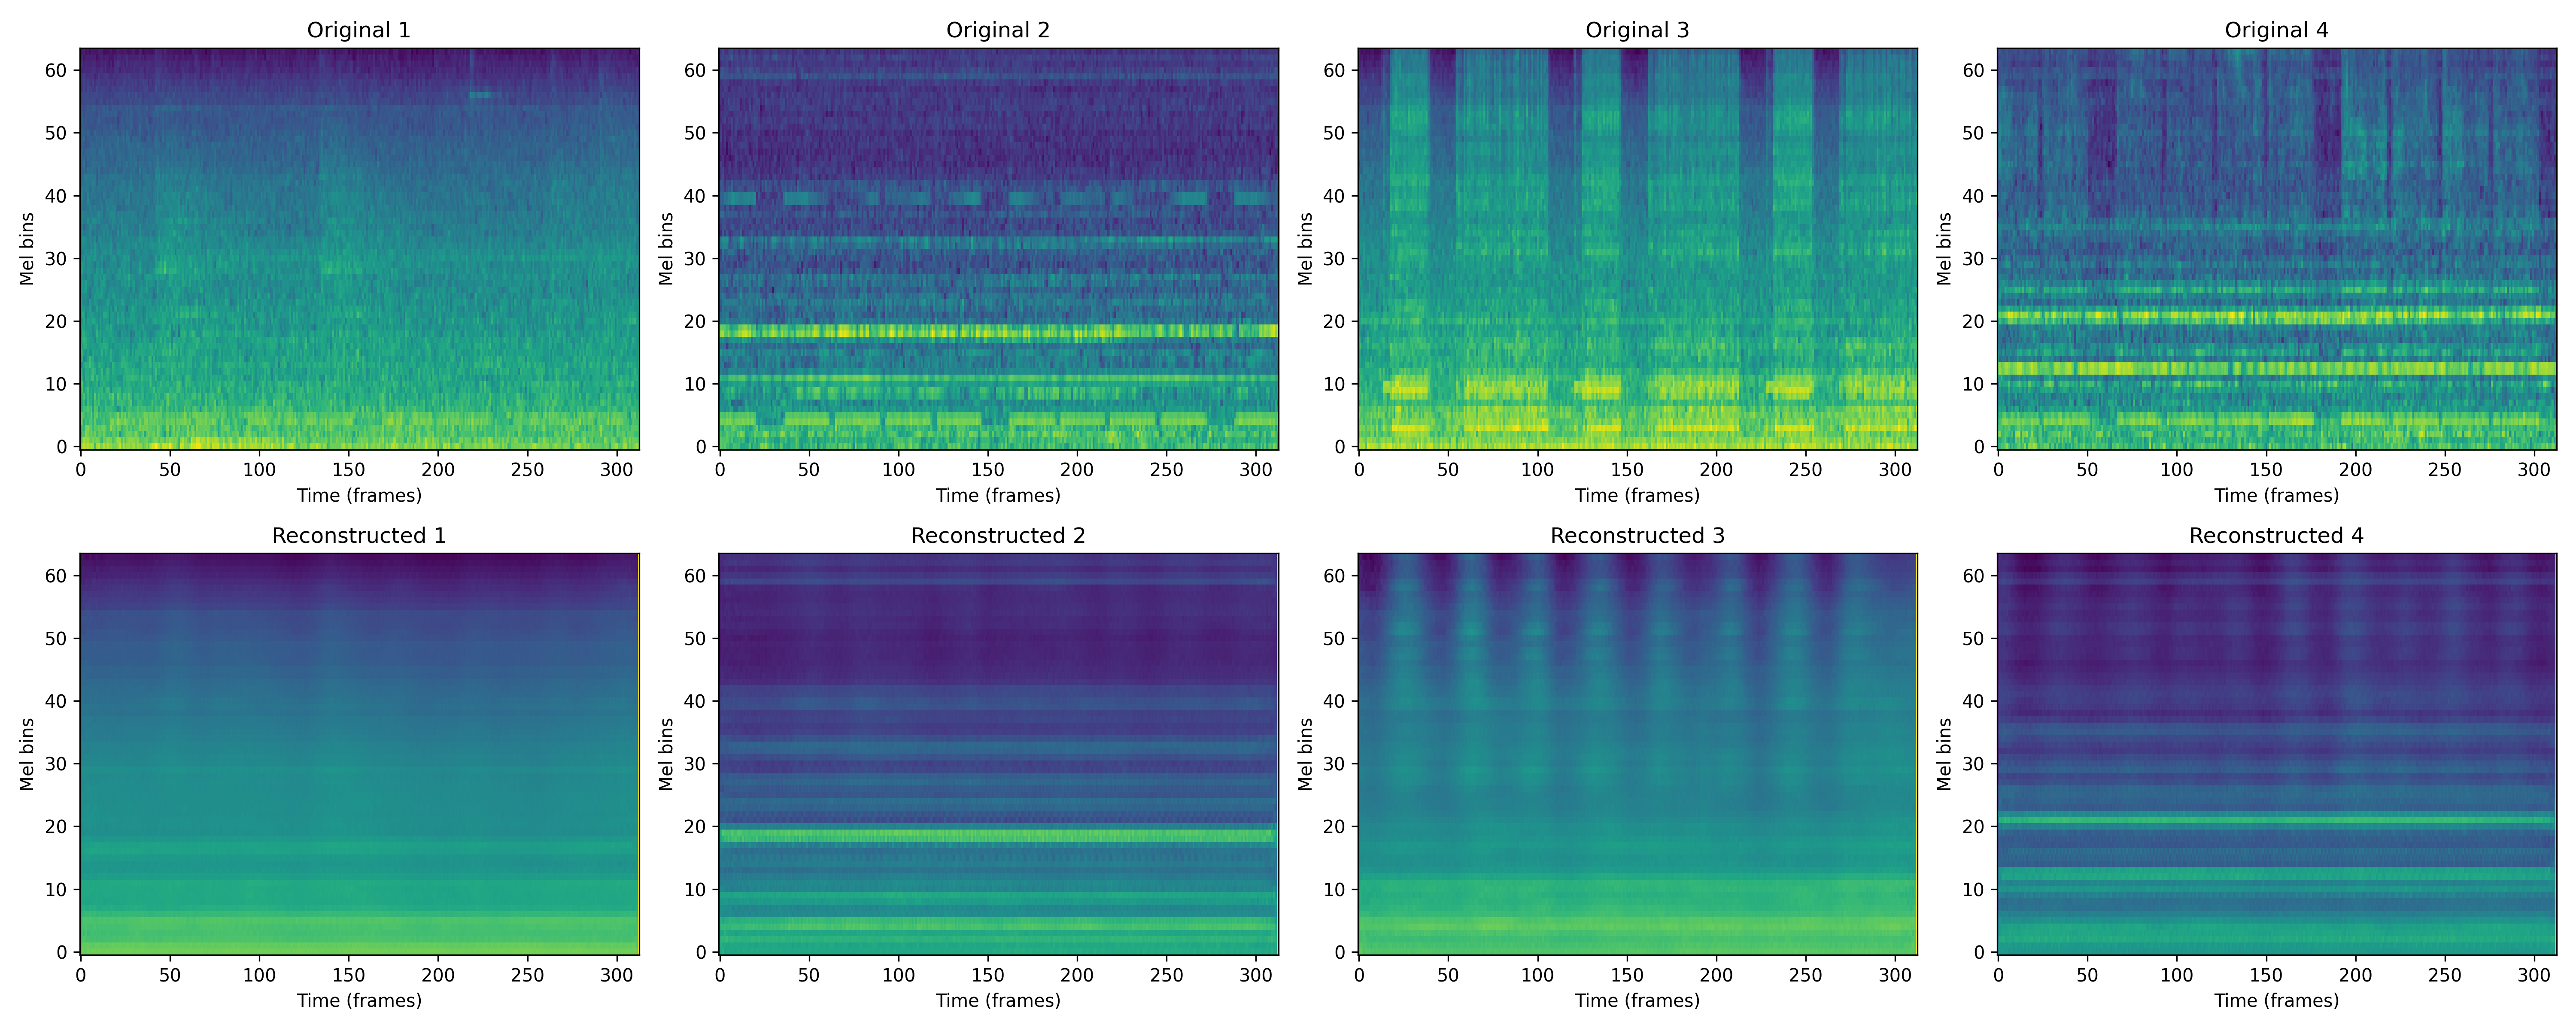
\includegraphics[width=\textwidth]{Figures/fig_reconstruction_examples_epoch24.png}
  \caption{Original (\emph{top}) versus reconstructed (\emph{bottom})
           log-Mel spectrograms produced by the CAE at epoch~24.
           Columns~1–2 are normal samples; Columns~3–4 are anomalous
           samples.  Normal inputs are faithfully reconstructed, whereas
           anomalies display spectral distortion, confirming the use of
           reconstruction error as an anomaly score.}
  \label{fig:recon_examples}
\end{figure}

Figure~\ref{fig:recon_examples} contrasts original and reconstructed
log-Mel spectrograms at epoch~24.  Normal inputs are reproduced almost
perfectly, whereas anomalous inputs incur visible spectral artefacts,
indicating higher reconstruction errors that are later exploited at
inference time.

% ..................................................................

\paragraph{Deep-SVDD.}
For the Deep-SVDD branch we adopt the soft-boundary objective.  
The feature extractor consists of three $3{\times}3$ convolutional
blocks (16-32-64 filters) followed by a fully connected layer that maps
to a \textbf{128-dimensional} embedding; all layers use ReLU activations
and $2{\times}2$ max-pooling.  

Training proceeds for \textbf{10 epochs} with Adam
($\alpha = 1\!\times\!10^{-4}$, batch size~64).
At the first forward pass, the hypersphere centre $c\!\in\!\mathbb{R}^{128}$
is initialised as the mini-batch mean; thereafter it is updated with a
moving average  
$c \leftarrow 0.9\,c + 0.1\,\bar{e}^{(t)}$,  
where $\bar{e}^{(t)}$ denotes the batch mean embedding at iteration~$t$.
The loss minimises the squared Euclidean distance
$\lVert e_i - c\rVert^{2}$ for each sample~$e_i$, thus compacting normal
embeddings around~$c$.  
A shorter training horizon suffices because the objective converges
quickly once the centre stabilises, and longer runs risk
hypersphere collapse.

\vspace{0.4em}
\noindent
\section{Results}
\label{sec:Results}

% The anomaly detection system achieved strong performance in identifying anomalous audio recordings of Slide Rail machines. Using a reconstruction error-based approach, the CAE model achieved the following metrics using a threshold of 0.12 determined through F1 optimization:

The proposed anomaly–detection pipeline attains competitive performance on the Slide-Rail subset of the ToyADMOS2 benchmark. Table \ref{tab:cae_vs_svdd} summarises the main quantitative findings, while Figure \ref{fig:Accuracy and loss plot} and \ref{fig:Reconstructed error plot} provide diagnostic visualisations that underpin our discussion.


% \begin{table}[H]
% \center
% \caption{Achieved metrics of model performance.}
% \begin{tabular}{l|l}
% \textbf{Metric}   & \textbf{Value} \\ \hline
%  Precision & 0.8864 \\ 
%  Recall &  0.9064 \\
%  F1-score & 0.8963 \\
%  AUC & 0.9008
% \end{tabular}
% \label{tab:Model results}
% \end{table}

\begin{table}[ht]
    \centering
    \caption{Comparison of CAE and Deep-SVDD on the slide-rail test set}
    \label{tab:cae_vs_svdd}
    \renewcommand{\arraystretch}{1.1}
    \begin{tabular}{lcccc}
        \toprule
        \textbf{Model} & \textbf{Precision} & \textbf{Recall} & \textbf{F1-score} & \textbf{AUC} \\
        \midrule
        CAE (tuned)   & 0.8864 & 0.9064 & 0.8963 & 0.9008 \\
        Deep-SVDD     & 0.7275 & 1.0000 & 0.8423 & 0.9552 \\
        \bottomrule
    \end{tabular}
\end{table}

The convolutional auto-encoder (CAE), tuned by maximising the validation F1-score, achieves an AUC of 0.9008 and an F1-score of 0.8963 at the optimum decision threshold.  In contrast, Deep-SVDD attains a marginally higher AUC of 0.9552 but at the cost of a markedly lower precision (0.7275), indicating a higher false-positive rate.  In an industrial quality-control setting—where false alarms lead to unnecessary downtime—the CAE therefore represents the more practical trade-off between sensitivity and specificity. 


\begin{figure}[H]
    \centering
    \subfigure[ROC characteristics of the SVDD model.]{
        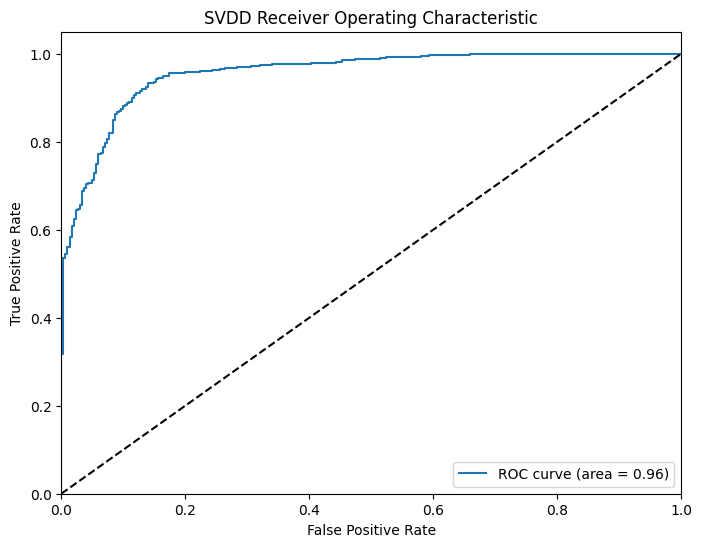
\includegraphics[width=0.45\textwidth]{Figures/svdd ROC.png}
        \label{fig:ROC SVDD}
    }
    \hspace{0.05\textwidth}
    \subfigure[ROC characteristics of the CAE model.]{
        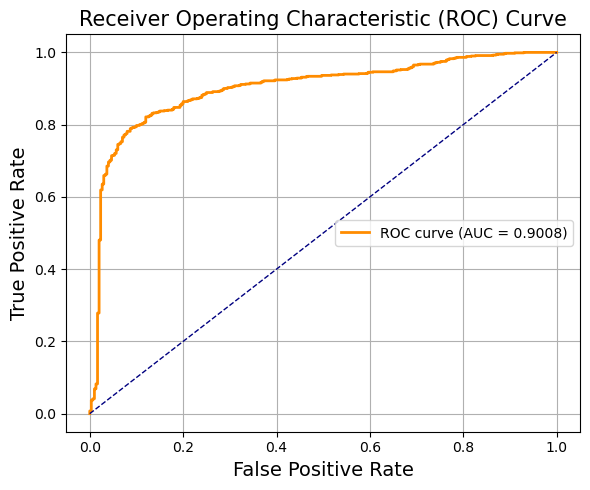
\includegraphics[width=0.4\textwidth]{Figures/ROC curve.png}
        \label{fig:ROC CAE}
    }
    \caption{Model performance.}
    \label{fig:Accuracy and loss plot}
\end{figure}

% Figure \ref{fig:ROC CAE} shows the ROC characteristics of the CAE model while Figure \ref{fig:ROC SVDD} shows the ROC characteristics of the SVDD Model. Overall, the performance of the model shows low false positive and false negative rates, which yields a good balance between precision and recall. This means that we are able to effectively detect anomalies while avoiding excessive false alarms.

% ---------- Results: ROC Analysis ----------

Figure~\ref{fig:ROC SVDD} depicts the the receiver–operating characteristic (ROC) of the
\textbf{Deep-SVDD} model, whereas Figure \ref{fig:ROC CAE} presents the ROC of the
\textbf{convolutional auto-encoder (CAE)}.
Both curves climb rapidly toward the upper-left corner, indicating low false–positive and false–negative
rates and, therefore, a favourable balance between precision and recall.
Closer inspection, however, reveals two nuances that match the quantitative findings in
Table~\ref{tab:cae_vs_svdd}:

\begin{itemize}
  \item \textbf{Steepness and stability (CAE, orange).}  
        The CAE ROC rises almost vertically and then hugs the left-hand axis,
        demonstrating robust discrimination across a broad range of operating
        thresholds.
        This geometry translates into a \textit{precision} of~$0.886$ and a
        \textit{recall} of~$0.906$ at the F$_1$-optimal decision boundary
        ($\text{threshold}=0.12$), yielding an $\text{AUC}=0.901$.
        Consequently, the CAE offers a generously wide ``safe zone’’ in which both
        Type-I and Type-II errors remain acceptably low—an attractive property for
        real-time deployment where threshold re-tuning is inevitable.

  \item \textbf{Higher plateau but concavity (SVDD, blue).}  
        Deep-SVDD attains a higher overall $\text{AUC}=0.955$, reflecting stronger
        rank-ordering ability.
        Nevertheless, its ROC exhibits a broader concave segment through the
        intermediate false-positive region, a signature of threshold instability.
        Numerically, this appears as a \textit{precision} of~$0.728$ despite
        perfect recall, implying that the model flags considerably more benign
        recordings as defective.
        From a decision-theoretic standpoint, such behaviour could lead to costly
        false alarms in an industrial monitoring scenario.
\end{itemize}

Taken together, the comparison shows that \textbf{Deep-SVDD excels in global ranking
(higher AUC), whereas the CAE delivers a more practical precision–recall trade-off
and greater threshold robustness}.
These observations align with the notebook’s per-epoch logs and the histogram of
reconstruction errors (Figure~\ref{fig:Reconstructed error plot}), corroborating that the CAE is the preferable choice when minimising false alarms is paramount, even if it
concedes a slight deficit in raw AUC.

The histogram of reconstruction errors presented in Figure \ref{fig:Reconstructed error plot} shows the separation between normal and anomalous instances. The distributions showed minimal overlap, with anomalous samples clustering toward higher error values. The 0.12 threshold clearly delineates the two classes.

\begin{figure}
    \centering
    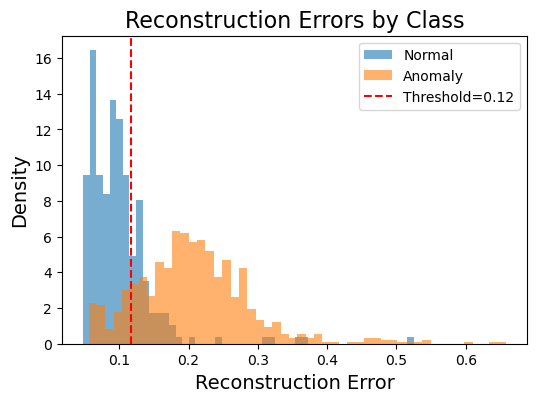
\includegraphics[width=0.8\linewidth]{Figures/Reconstruction error plot.png}
    \caption{Histogram over RMS values}
    \label{fig:Reconstructed error plot}
\end{figure}
\section{Discussion}
\label{Sec:Discussion}

The model’s strong performance metrics confirm the efficacy of autoencoders architectures for anomaly detection tasks. It shows that the model generalizes well from training exclusively on normal data, successfully detecting unseen anomalies during testing. The last is key for developing cost-effective solutions as the collection of anomalous samples may be considerably expensive.

The results also highlight the importance of threshold selection. An F1-optimized threshold yielded a balanced trade-off between precision and recall. However, for industrial applications other approaches may be explored, specially those taking into account the difference between the cost of a false alarm (false positive) and a non identified anomaly (false negative). 

Despite these promising results, one must note the limitation due to the reduced experiment's scope. The evaluation was focus to the Slide Rail machine type so generalization to other machine types is not guaranteed.
\section{Conclusion}
\label{Sec:Conclusion}

This work presented a fully unsupervised pipeline for acoustic anomaly detection, using only normal data during training and leveraging reconstruction error as the detection signal. The method proved highly effective in distinguishing between normal and anomalous recordings for Slide Rail machines, achieving a ROC AUC of 0.9008 and an F1 score of 0.8963. The results emphasize the viability of such techniques in real-world applications where anomalies are rare and cost to collect. 






\phantomsection
\addcontentsline{toc}{section}{References}
\begin{thebibliography}{99}

\bibitem{purohit2019mimii}
H. Purohit, Y. Koizumi, N. Harada, and Y. Mitsufuji, 
``MIMII Dataset: Sound Dataset for Malfunctioning Industrial Machine Investigation and Inspection,'' 
in \textit{Proc. IEEE Workshop on Applications of Signal Processing to Audio and Acoustics (WASPAA)}, 2019, pp. 249--253. 
\textit{doi}: \href{https://doi.org/10.1109/WASPAA.2019.8937164}{10.1109/WASPAA.2019.8937164}.

\bibitem{purohit2019improving}
H. Purohit, K. Imoto, Y. Koizumi, N. Harada, and Y. Mitsufuji, 
``Improving Unsupervised Anomalous Sound Detection with Auxiliary Bi-level Information,'' 
in \textit{Proc. DCASE Workshop 2019}, New York University, NY, USA, 2019, pp. 21--25. 
\textit{Online}: \url{https://dcase.community/documents/workshop2019/proceedings/DCASE2019Workshop_Purohit_21.pdf}

\bibitem{CNN}
    Geeksforgeeks (2025)
    \textit{Introduction to Convolution Neural Network}.
    Available from: \href{https://www.geeksforgeeks.org/introduction-convolution-neural-network/}{Geeksforgeeks}
    (Fetched: 9. May 2025)

\end{thebibliography}


\end{document}